\documentclass[twocolumn]{IEEEtran} 

\usepackage[utf8]{inputenc}
\usepackage{amstext}
\usepackage{amsmath}
\usepackage{graphicx}
\usepackage{textcomp}
\usepackage{float}
\usepackage{varioref}
\usepackage{fancyref}
\usepackage{caption}
\usepackage{subcaption}
\usepackage{comment}
\usepackage{hyperref}
\usepackage{epstopdf}

\vrefwarning

\usepackage{graphicx}

\begin{document}

\title{Comparison Between Swish and Backboard Shots}

\author{James Jang and Filippos Lymperopoulos}

\markboth{ModSim Mechanics Final Project, Vol. 1, No.
1}{ModSim Mechanics Final Project, Vol. 1, No.
1}

\maketitle
\begin{abstract} 

This paper will theoretically and experimentally develop an analysis of the motion and behavior of the basketball and further determine optimal scenarios of shooting with or without the backboard in 2D and 3D. Hence, taking into account spin and the effect of drag and the Magnus force, we can study swish and backboard shots.

\end{abstract}

\begin{keywords}
basketball, spin, Drag force, Magnus force, angular velocity, collision
\end{keywords}

\section{Introduction}

Basketball started as a winter exercise for football players in 1891. It has since then become one of the most popular sports in the world. The main goal of the game is to score and a player can do that by shooting a ball into a basket that is positioned at a height of 10ft off the ground to score. There are several ways to put the ball into the basket such as layups, dunk shots and bank shots. When shooting from a distance, players tend to shoot jump shots. Interesting thing to note is that when these shots away from the basket tend to mostly be swishes instead of banked shots. The backboard seems to exist so that players can hit the ball off of it for assistance. This paper will be modeling the shooting of a basketball that includes the interaction between the ball and the backboard and ball and the rim. Using the model we will be able to determine why players tend to shoot swishes. We will first describe the physics of the model and go on to cover the limitations of the model. Finally the results will be discussed and their implications.

\section{Modeling the shooting of the ball}

\subsection{Abstraction of the Shooting}

\begin{figure}[!ht]
\includegraphics[height=2in]{basketball}
\caption{Illustration of the abstraction of the basketball's motion in two dimensions. The basketball is abstracted as a single rigid body. An initial speed and angle of the projectile is given at the first stage of the motion, the flight. The basketball is assumed to experience the force of gravity $\emp F_g$, a drag force $\emp F_d$ and a Lift force $\emp F_L$, while it is back-spinning (indicated by $\vec \omega$) and moving at the direction of the linear velocity $\emph v$.}
\end{figure}

When the ball is shot there are three main phases, the flight, the backboard interaction and the rim interaction. For the sake of simplicity, we will initially use a 2 dimension to explain the model.

Looking into the first phase of the flight, the ball is given an initial velocity in the direction of the initial angle of the projectile ($\theta$), as shown in Figure 1. The ball leaves the shooter's hand with a given angular velocity. Taking into account that the there are three kinds of forces that act upon the ball, we can derive accurate equations of motion for the ball. More precisely, the forces include the force of gravity $F_g$, the force of drag $F_d$ and the lift force $F_L$. The equations we get are
\begin{align}
\vec F_g &= -m g\\
\vec F_d &= -\frac{1}{2} C_d A v^2\\
\vec F_L &= s (\vec \omega \times \vec v)
\end{align}

In the case of gravity, $\emph g$ is used as 9.81 $ms^-2$, while in the drag force equation, $C_d$ represents the coefficient of drag, while A is equal to the area of the ball, followed by the velocity it travels with,$\vec v$. Finally, the force of lift equals to the cross product of the angular ($\vec \omega$) and linear velocity ($\vec v$), along with the lift constant $\emp s$. This constant is assumed to be close to zero, i.e. 0.02. The force of gravity acts in the negative y-direction. The force of drag always acts parallel to velocity in the negative direction. The Magnus force always acts perpendicular to the velocity. Hence, the following expression of the ball's acceleration can be derived.
\begin{align}
F_{total} &= F_d + F_L -mg
\end{align}
Yielding the following:
\begin{align}
a &= \frac{F_d}{m} + F_L -g\\
a &= \frac{C_d Av^2+2 s (\vec \omega \times \vec v)-2g}{2m}
\end{align}
\begin{figure}[!ht]
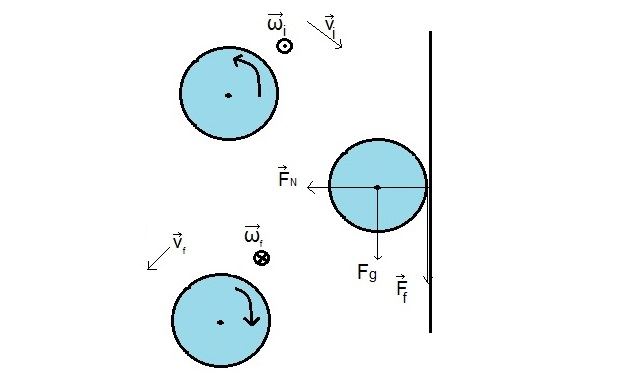
\includegraphics[height=2in]{basket}
\caption{Illustration of the abstraction of the basketball's motion in two dimensions during the collision with the board, the second phase of the motion. The velocity $\vec v$ and $\vec \omega$ are changed after the collision of the ball on the board. The force of gravity $\emp F_g$, a normal force $\emp F_N$ and a frictional force $\emp F_f$ act on the ball during contact with the board, where no spin takes place. After the collision, the ball moves with different velocities  $\vec v_f$ and $\vec \omega_f$, whose directions have been altered.}
\end{figure}

The second phase of the motion involves the ball-backboard interaction. In that case, the velocity and the angular velocity change states. The change in velocity that is parallel to the surface of the interaction is modeled by the coefficient of restitution ($C_r$). When the ball hits a surface, the slipping of the ball from the angular velocity causes the friction force to act on the ball. This friction force applies torque on the ball, changing the angular velocity and the velocity parallel to the surface of the interaction. Because the initial and final velocities are known, the change in momentum is also known (impulse). This is very important because the frictional impulse is dependent on the the total impulse. The backboard is on the y-axis so this makes the collision simpler. The relative equations are given below.
\begin{align}
v_{xnew} &= -v_x C_r\\
I_n &= mv_x (1+C_r)\\
I_f &= \mu_s (I_n)\\
v_{ynew} &= \frac{I_f}{m} +v_y
\end{align}

More precisely, $C_r$ is the coefficient of restitution and $\mu_s$ is the coefficient of static friction. $I_n$ is the total impulse and $I_f$ is the frictional impulse. 

The interaction between the ball and the rim is a little more complicated because the parallel and the normal planes are not constant and change depending where the ball hits the rim. A normal vector can be created from the center of the ball to the point of contact on the rim. This normal vector further defines the plane of the surface. For our model, the interaction with the rim was not the main part of the model so the interaction was simplified by assuming that angular velocity does not exist. Thus, the coefficient of restitution to change the velocity.
\begin{align}
v_{xnew} &= -v_x C_r (\frac{v_x}{\hat V})\\
v_{ynew} &= -v_y C_r (\frac{v_y}{\hat{V}})\\
v_{znew} &= -v_z C_r (\frac{v_z}{\hat{V}})
\end{align}

\begin{figure}[!ht]
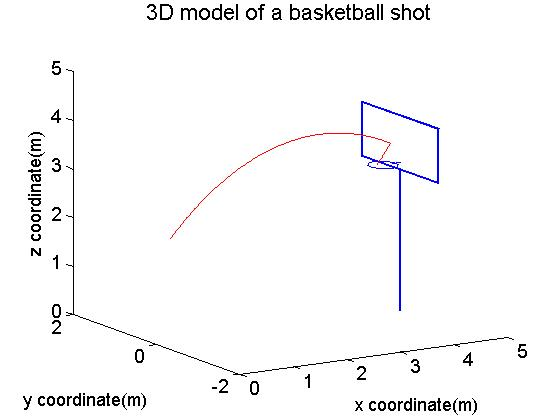
\includegraphics[height=2.5in,width = 3.5in]{3Dbasketballshot}
\caption{3D depiction of a basketball shot interacting with backboard}
\end{figure}
\section{Limitation}
An interesting limitation in our model is the interaction between the rim and the ball. The model describes a simplified interaction with the rim. 

\section{Validation}
Taking into account the fact that the angle from which the shot was taken could distort the measured results, a camera was positioned at the same height as the basket and both swish and bank shots were monitored. Our goal was to see how accurate our model was in relation to real life shots. 
\begin{figure}[!ht]
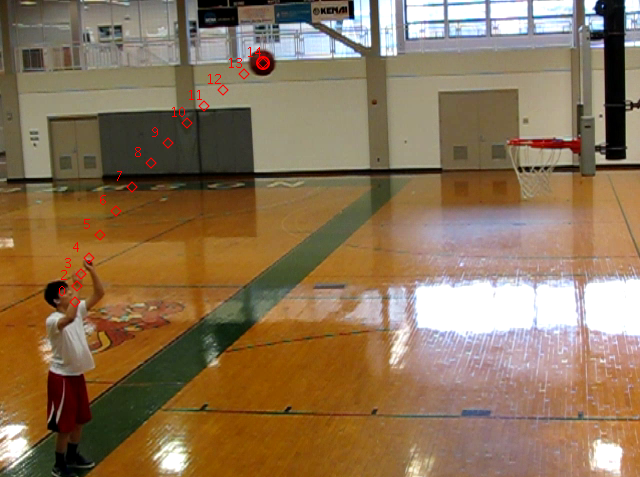
\includegraphics[height=2.6in]{1}
\caption{Capture of the shot made along with the points tracked.}
\end{figure}

We wanted to see the proximity that the modelled trajectory we generated, mapped the actual trajectory of the basketball. For the specific validation, we were bounded to test shots made in the plane that was parallel from the side of the backboard from the free-throw line - other words, in two dimensions.

In Figure 5, two trajectories of straight swish shots are presented. The dotted line indicates the experimental data received from the software Tracker we used. The red line depicts the theoretical data produced by the second order differential equation solver implemented. The two distinct parts of the motion - the flight and backboard collision - seem to match very well, validating our model.
\begin{figure}[!ht]
\includegraphics[height=2.5in,width = 3.8in]{swishshot1}
\caption{Analysis of the swish shot case.}
\end{figure}

Moreover, the projectile that results from the bank shot, limited in the plane that cuts through the middle of a basket, given both from the second order differential equation solver and the tracking software, seem to continue at a relative similar path. No interaction between the ball and the rim took place, and the ball got into the basket in both cases. The backboard collision comparison between the theoretical and the experimental data further validate our model, as shown in the figure that follows.
\begin{figure}[!ht]
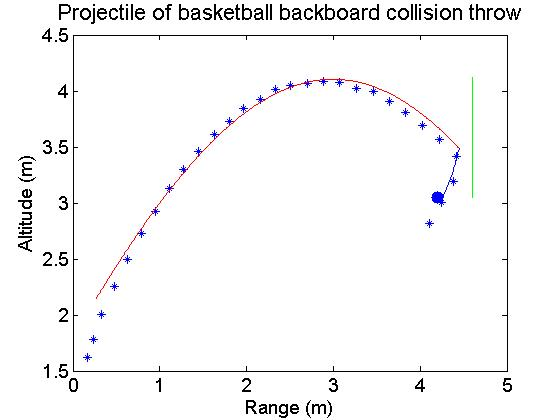
\includegraphics[height=2.5in,width = 3.5in]{newBackboard}
\caption{Bank shot diagram for theoretical and experimental data.}
\end{figure}
As a result, the two experiments indicated validate our model, confirming that the trajectory generated by the differential equation solver coincides with that of an actual shot.

\section{Figures of Merit}

With a strong validation for the flight of the basketball, and the interaction between the ball and the backboard our model is validated. More precisely, angular velocity is very important in determining the trajectory of the ball in flight and after the collision. It is recommended for all players to shoot with a backspin because that softens the interaction between the rim and the ball and also shoots the ball downward toward the basket when the ball hits the backboard, rather than bouncing erratically back out. We decided to test how much impact initial angular velocity, $\vec \omega$, had, if the shot was made. In essence, $\phi$ does not affect our model very much. It was added as a 3D parameter and the graph was more easily interpreted when $\phi$ was held constant. Four graphs with different initial angular velocities -10 rads$^{-1}$ (normal topspin), 0 rads$^{-1}$ (no spin), 10 rads$^{-1}$ (normal backspin), 30 rads$^{-1}$ (intense backspin) were generated to analyze and compare the effect of spin.

\begin{figure}[!ht]
\includegraphics[height=2.5in,width = 3.8in]{topspin}
\caption{Graph of basketball shots that were made when $\phi$ was held constant with initial angular velocity of 10 rad/s ( topspin}
\end{figure}

As the initial launch angle increases, the initial velocity needed to make the shot goes up, drastically. The banked shots require a larger initial velocities, as expected. There is, hence, a definite gap between the two cases. While the difference is not huge, the area of the swish shots seems to be bigger, which shows that swish shots have higher probability of going in.

\begin{figure}[!ht]
\includegraphics[height=2.5in,width = 3.8in]{0spin}
\caption{Graph of basketball shots that were made when $\phi$ was held constant with no initial angular velocity}
\end{figure}

The graph with no spin looks very similar to the graph with the -10 rads$^{-1}$ topspin. Yet, the steepness of the curve of the cluster of points differs, and in that case it's lower.

\begin{figure}[!ht]
\includegraphics[height=2.5in,width = 3.8in]{normalomega}
\caption{Graph of basketball shots that were made when $\phi$ was held constant with the initial angular velocity of 10 rad/s}
\end{figure}

The initial angular velocity of 10 rads$^{-1}$ is approximately the ideal amount of backspin applied in an ideal shot. The difference in the thickness of the bands is pretty significant compared to the two previous graphs. This shows that basketball shots with a certain amount of backspin have a higher chance of going into the basket than shots with a given amount of topspin or no spin at all.

\begin{figure}[!ht]
\includegraphics[height=2.5in,width = 3.8in]{30backspin}
\caption{Graph of basketball shots that were made when $\phi$ was held constant with initial 30 rad/s}
\end{figure}

In all of the graphs above, the red circles represent the banked shots that went through the hoop and the blue circles represent the swish shots that went through the basket. We can see that the Magnus force has a great impact for different angular velocities. With an amount of topspin, the Magnus force acts perpendicular to the velocity, resulting in a "pulling down" effect of the ball to the ground. As the initial backspin increases, the curves of the blue and red clusters become flatter. The curve seems to reverse when the backspin increases, which can be shown in the final graph on Figure 10. An interesting thing to note is that when the initial angular velocity is 30 rads$^{-1}$, which theoretically is very hard to generate for a human to shoot, the only shots that are shown in the graph are all swishes. Within the scale of the graph, there are no banked shots, which means it requires higher velocity to make such shots. This is because the Magnus force generated by backspin stabilizes the shots.

The difference in the thickness of the band is pretty significant between the topspin graph and normal backspin graph. As a result, players definitely have a higher chance of making their shots if they put backspin on the ball.

In all of the graphs, there are outliers that are separated from the cluster. There are also empty areas within the cluster. This is due to the ball hitting the rim and bouncing off and either going into the basket or going out of the basket. The outliers around the bottom of the chunks are due to the ball bouncing off the front of the rim and the outliers around the top of the chunks are due to the ball bouncing off the back of the rim.


\section{Conclusion}

Our model shows that Magnus force seems to have a huge impact on the shots. If a player somehow shoots with a topspin, then they must exert more force to generate higher initial velocities. If the curve of the red and blue clusters tends to be flatter with normal initial backspin and, hence, if the curves are flatter then the players do not have to exert a lot of force to make their shots in. The initial velocities tends to stay between 7 and 7.5, until around when $\theta$ equals 60. This explains why players would want to shoot the basketball with a decent amount of backspin because that allows the players to still make in their shots even when they vary the launch angle. The difference in the thickness of the band also shows that players have higher chance of making the shots when they shoot with backspin on the ball. Consistency is very important when shooting and our results show that shots with backspin definitely increases the chance of scoring. Some of the important analysis we would like to do in the future is focus on solely the backboard interaction and observe how much the initial velocities impact the basketball shot. This would require eliminating the effect of the Magnus force in the flight of the ball.


\section*{Acknowledgments}
We would like thank Mark Somerville, the NINJAS, and, especially Adit Dhanushkodi, for all of their guidance for working on the physics and modeling our model as well as writing our paper. 

\nocite{*}
\bibliographystyle{IEEE}

%%%%%%%%%%%%%%%%% BIBLIOGRAPHY %%%%%%%%%%%%%%%%%%%%%%%%
\begin{thebibliography}{1}
\bibitem{ScienceDaily} Creighton \ University\ , ``Basketball: The physics of the 3-point shot''  {\it ScienceDaily}, March 21, 2014.
\bibitem{Unknown} Rod Cross, {\it BALL TRAJECTORIES},Web., June 2011, 2014.
\bibitem{Real World Physics Problems} The Physics of Basketball, {\it Physics of Basketball}, Web., May 05 2014.
\bibitem{ScienceDaily} North Carolina State University, {\it Nothing But Net: The Physics Of Basketball Free Throws}, Web., May 05 2014.
\end{thebibliography}

\end{document}

--------------------------------------------------------------------------------